\subsection{Proving the Quadratic Formula}
\begin{definition}[Quadratic]
	$$f(x) = ax^2 + bx + c = 0$$
	$$ax^2 + bx + c = 0$$
\end{definition}

\subsubsection{Proof}
$$ax^2 + bx \qquad + c = 0$$
$$a(x^2 + \frac{b}{a}x \quad) \quad + c = 0$$
\begin{center}
	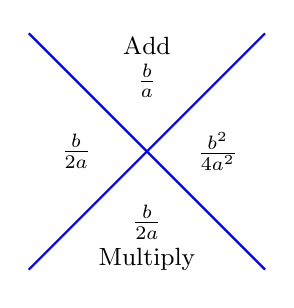
\begin{tikzpicture}[scale=1.5, auto, >=stealth]
		\draw[thick, blue] (-1, 1) -- (1, -1);
		\draw[thick, blue] (-1, -1) -- (1, 1);
		\node at (0, 0.6) {$\frac{b}{a}$};
		\node at (0, -0.6) {$\frac{b}{2a}$};
		\node at (-0.6, 0) {$\frac{b}{2a}$};
		\node at (0.6, 0) {$\frac{b^2}{4a^2}$};
		\node at (0, 0.6) [above=6pt] {\small Add};
		\node at (0, -0.6) [below=6pt] {\small Multiply};
	\end{tikzpicture}
\end{center}
$$a(x^2 + \frac{b}{a}x + \frac{b^2}{4a^2}) \quad + c = 0$$
$$a(x^2 + \frac{b}{a}x + \frac{b^2}{4a^2}) - \frac{b^2}{4a^2} + c = 0$$
$$a(x^2 + \frac{b}{a}x + \frac{b^2}{4a^2}) - \frac{b^2}{4a^2} + \frac{4ac}{4a}$$
$$a(x + \frac{b}{2a})^2 = \frac{b^2}{4a} - \frac{4ac}{4a}$$
$$a(x + \frac{b}{2a})^2 = \frac{b^2 - 4ac}{4a}$$
$$(x + \frac{b}{2a})^2 = \frac{b^2 - 4ac}{4a^2}$$
$$\sqrt{(x + \frac{b}{2a})^2} = \pm \sqrt{\frac{b^2 - 4ac}{4a^2}}$$
$$x + \frac{b}{2a} = \pm \frac{\sqrt{b^2 - 4ac}}{2a}$$
$$x = - \frac{b}{2a} \pm \frac{\sqrt{b^2 - 4ac}}{2a}$$
$$x = -b \pm \frac{\sqrt{b^2 - 4ac}}{2a}$$
